\documentclass{article}
\usepackage{graphicx}
\usepackage[table]{xcolor}
\usepackage[utf8]{inputenc}
\usepackage{siunitx}
\usepackage[american,siunitx]{circuitikz}
\usepackage{amsmath}
\usepackage{svg}
\usepackage{booktabs}
\usepackage{float}
\usepackage{xparse, xfp}
\usepackage{multirow}
\usepackage{tikz}
\usepackage{karnaugh-map}
\usepackage{pdfpages}
\usepackage{hyperref}
\hypersetup{
    colorlinks=true,
    linkcolor=blue,
    filecolor=magenta,      
    urlcolor=cyan,
}
\usetikzlibrary{calc}
%\usepackage[landscape]{geometry}
\renewcommand{\thesubsection}{\thesection.\alph{subsection}}
\newcommand{\equal}{=}
\newcommand{\greyrule}{\arrayrulecolor{black!30}\midrule\arrayrulecolor{black}}
\makeatletter
\newcommand\currcoor{\the\tikz@lastxsaved,\the\tikz@lastysaved}
\makeatother
\newcolumntype{:}{@{\hskip\tabcolsep\color{black!30}\vrule\hskip\tabcolsep}}

\ExplSyntaxOn
\NewExpandableDocumentCommand \groupify { O{\,\allowbreak} m m }
  { \jakob_groupify:nnn {#1} {#2} {#3} }
\cs_new:Npn \jakob_groupify:nnn #1 #2 #3
  { \__jakob_groupify_loop:nnw { 1 } {#2} #3 \q_recursion_tail {#1} \q_recursion_stop }
\cs_new:Npn \__jakob_groupify_loop:nnw #1 #2 #3
  {
    \quark_if_recursion_tail_stop:n {#3}
    \exp_not:n {#3}
    \int_compare:nNnTF {#1} = {#2}
      { \__jakob_groupify_sep:n }
      { \exp_args:Nf \__jakob_groupify_loop:nnw { \int_eval:n { #1+1 } } }
          {#2}
  }
\cs_new:Npn \__jakob_groupify_sep:n #1 #2 \q_recursion_tail #3
  {
    \tl_if_empty:nF {#2} { \exp_not:n {#3} }
    \__jakob_groupify_loop:nnw { 1 } {#1}
    #2 \q_recursion_tail {#3}
  }
\ExplSyntaxOff

\title{ECE 2300L\\Digital Logic Design Laboratory\\\,\\Experiment 11\\\,\\Report}
\author{Choi Tim Antony Yung}
\begin{document}
\maketitle

\thispagestyle{empty}
\setcounter{page}{0}

\newpage

\section*{State Diagram}
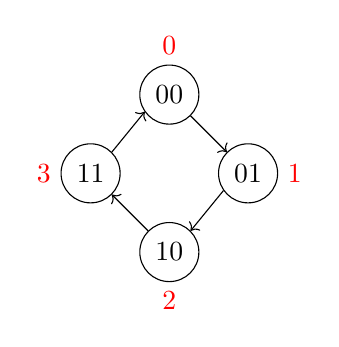
\begin{tikzpicture}
  \node(a)[draw,circle,minimum size=0.75cm,inner sep=0pt] at (0,0) {$00$};
  \node(b)[draw,circle,minimum size=0.75cm,inner sep=0pt] at (1,-1) {$01$};
  \node(c)[draw,circle,minimum size=0.75cm,inner sep=0pt] at (0,-2) {$10$};
  \node(d)[draw,circle,minimum size=0.75cm,inner sep=0pt] at (-1,-1) {$11$};
  \draw [->] (a.315) -- (b.135);
  \draw [->] (b.215) -- (c.45);
  \draw [->] (c.135) -- (d.315);
  \draw [->] (d.45) -- (a.215);
  \draw[color=red] (a.90) node[above]{0};
  \draw[color=red] (b.0) node[right]{1};
  \draw[color=red] (c.270) node[below]{2};
  \draw[color=red] (d.180) node[left]{3};
\end{tikzpicture}

\section*{State Table}
\begin{table}[H]
  \begin{tabular}{cc|cc|cc}
      \toprule
      $A$&$B$&$A^+$&$B^+$&$T_A$&$T_B$\\
      \midrule
      0&0&0&1&0&1\\
      0&1&1&0&1&1\\
      1&0&1&1&0&1\\
      1&1&0&0&1&1\\
      \bottomrule
  \end{tabular}
\end{table}

\section*{Truth Table}
\begin{table}[H]
  \begin{tabular}{cc|c}
      \toprule
      $A$&$B$&$T_A$\\
      \midrule
      0&0&0\\
      0&1&1\\
      1&0&0\\
      1&1&1\\
      \bottomrule
  \end{tabular}
  \quad
  \begin{tabular}{cc|c}
    \toprule
    $A$&$B$&$T_B$\\
    \midrule
    0&0&1\\
    0&1&1\\
    1&0&1\\
    1&1&1\\
    \bottomrule
\end{tabular}
\end{table}

\section*{Karnaugh Maps}
\begin{table}[H]
  \begin{tabular}{cc}
    \begin{karnaugh-map}*[2][2][1][$B$][$A$]
      \minterms{1,3}
      \implicant{1}{3}
    \end{karnaugh-map}
    &
    \begin{karnaugh-map}*[2][2][1][$B$][$A$]
      \minterms{0,1,2,3}
      \implicant{0}{3}
    \end{karnaugh-map}
    \\
    $T_A=B$&$T_B=1$\\
  \end{tabular}
\end{table}

\section*{Schematic}

\begin{center}
    \begin{circuitikz}
      \draw (0,0) node[dipchip,num pins=8,hide numbers,external pins width=0.0](decoder){};
      \draw (decoder.east) -- ++(0.5,0) node[above]{$a-g$} -- ++(0.5,0) node[seven segment val=8 dot none box on, anchor=west]{};
      \draw (decoder.bpin 1) node[right]{6} -- ++(-0.5,0) coordinate(d3) node[above]{$d_3$};
      \draw (decoder.bpin 2) node[right]{2} -- ++(-0.5,0) coordinate(d2) node[above](d2){$d_2$};
      \draw (decoder.bpin 3) node[right]{1} -- ++(-0.5,0) node[above]{$d_1$};
      \draw (decoder.bpin 4) node[right]{7} -- ++(-0.5,0) node[above]{$d_0$};
      \draw (decoder.bpin 1) ++(-0.5,0) -- ++(-0.5,0) -- (\currcoor|-decoder.bpin 2) -- ++(0,-0.2) node[tlground]{};
      \draw (decoder.bpin 2) ++(-0.5,0) -- ++(-0.5,0);
      \draw (decoder.bpin 3) ++(-0.5,0) -- ++(-1,0) node[flipflop JK, anchor=pin 6](JKA){} node[below]{A};
      \draw (decoder.bpin 4) ++(-0.5,0) -- ++(0,-3.5) -- ++(-1,0) node[flipflop JK, anchor=pin 6](JKB){} node[below]{B};
      \draw (JKA.pin 1) to[crossing] (JKA.pin 3) node[left]{$T_A$} -- ++(0,-1) -- (\currcoor-|JKB.pin 6) -- (JKB.pin 6);
      \draw (JKB.pin 1) node[vcc]{5V} node[left]{$T_B$} to[crossing] (JKB.pin 3);
      \draw (JKB.pin 2) -- ++(-1,0) -- (\currcoor|-JKA.pin 2) node[circ](clk){} to[R=\SI{1}{\kilo\ohm}] ++(0,1.5) node[vcc]{5V};
      \draw (JKA.pin 2) -- ++(-1,0);
      \draw (clk) ++(-1.5,0) node[ground]{} to[nopb] (clk);

      % pinout
      \draw [color=red]
      (JKA.bpin 1) ++(0.3,0) node[right]{14}
      (JKA.bpin 2) ++(0.3,0) node[right]{1}
      (JKA.bpin 3) ++(0.3,0) node[right]{3}
      (JKA.bpin 4) ++(-0.3,0) node[left]{13}
      (JKA.bpin 6) ++(-0.3,0) node[left]{12}
      (JKB.bpin 1) ++(0.3,0) node[right]{7}
      (JKB.bpin 2) ++(0.3,0) node[right]{5}
      (JKB.bpin 3) ++(0.3,0) node[right]{10}
      (JKB.bpin 4) ++(-0.3,0) node[left]{8}
      (JKB.bpin 6) ++(-0.3,0) node[left]{9}
      ;
    \end{circuitikz}
\end{center}

\newpage

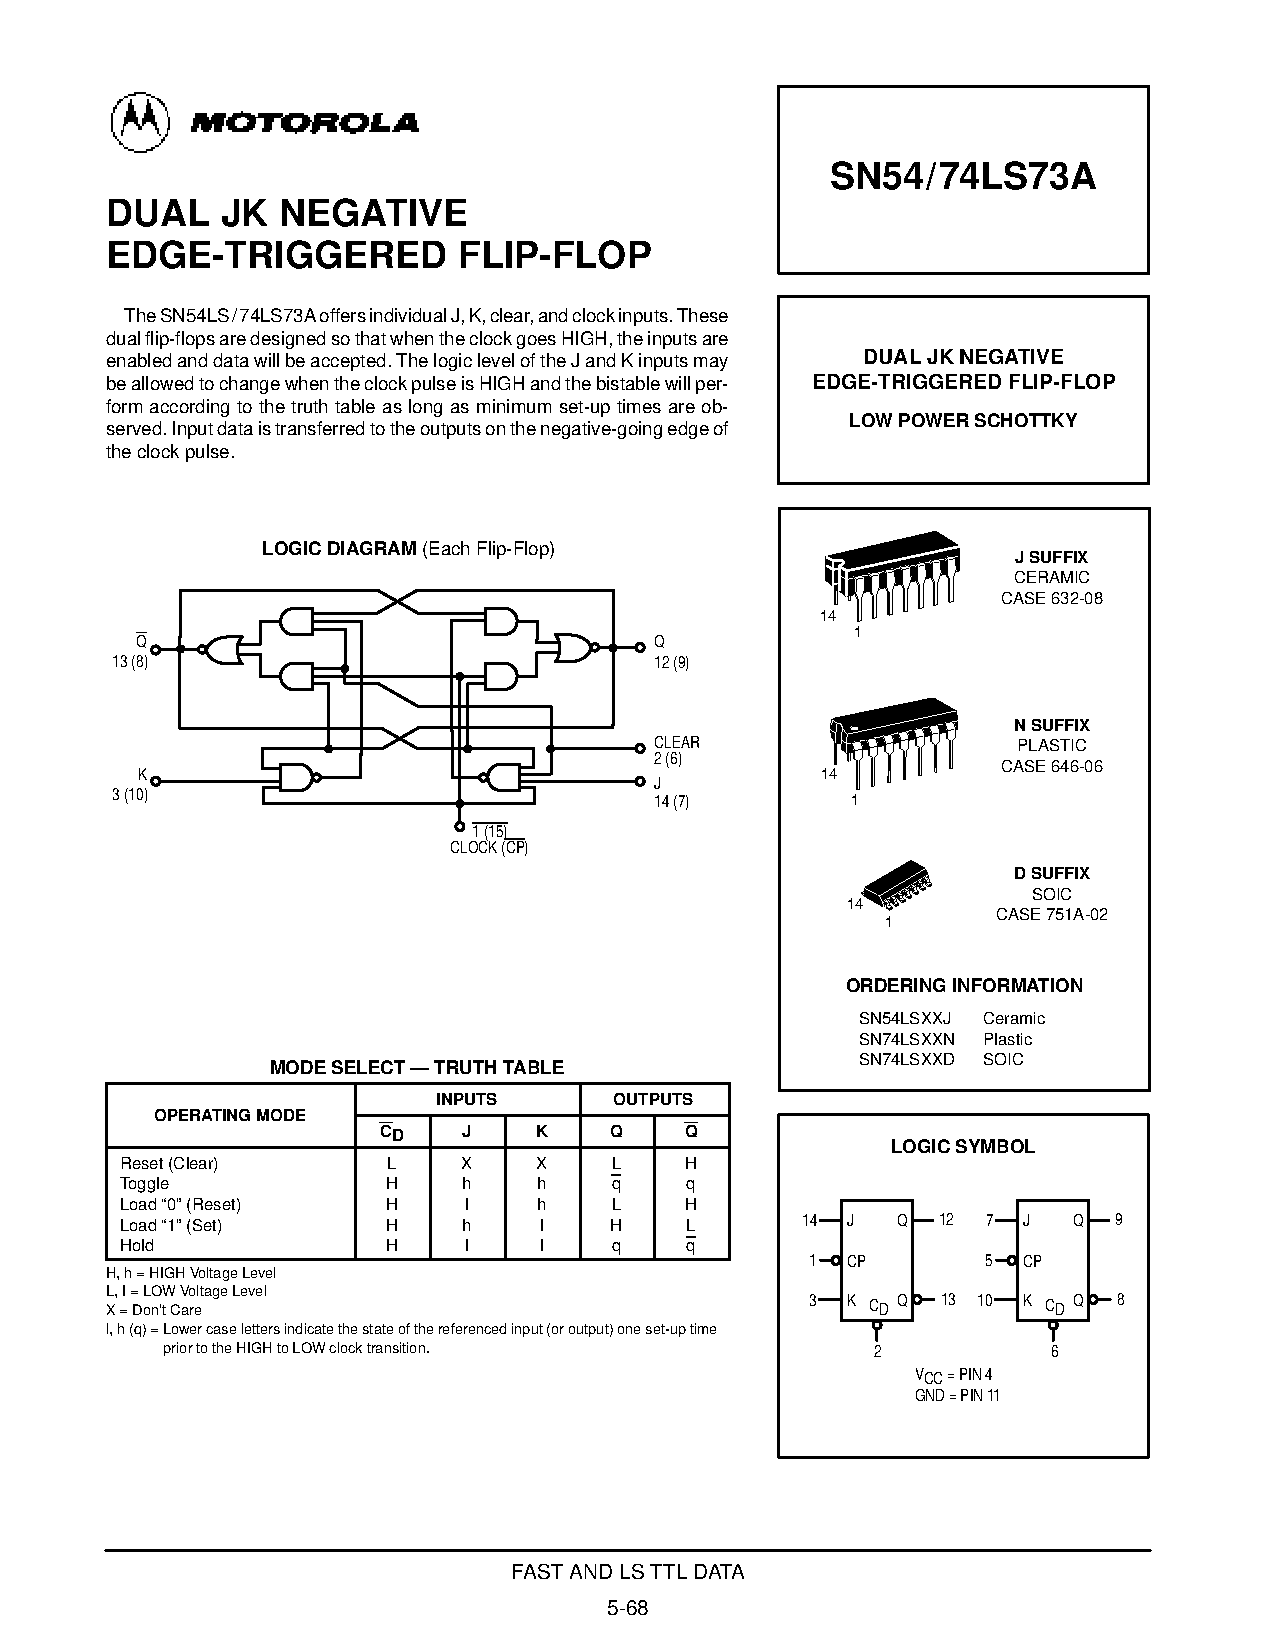
\includepdf[page={1}]{7473}

\newpage

\section*{Demo}
A video demonstration can be found \href{https://photos.app.goo.gl/729cwgJ9mkX1yE7Z6}{here} at \url{https://photos.app.goo.gl/729cwgJ9mkX1yE7Z6}
\begin{figure}[ht!]
  \centering
  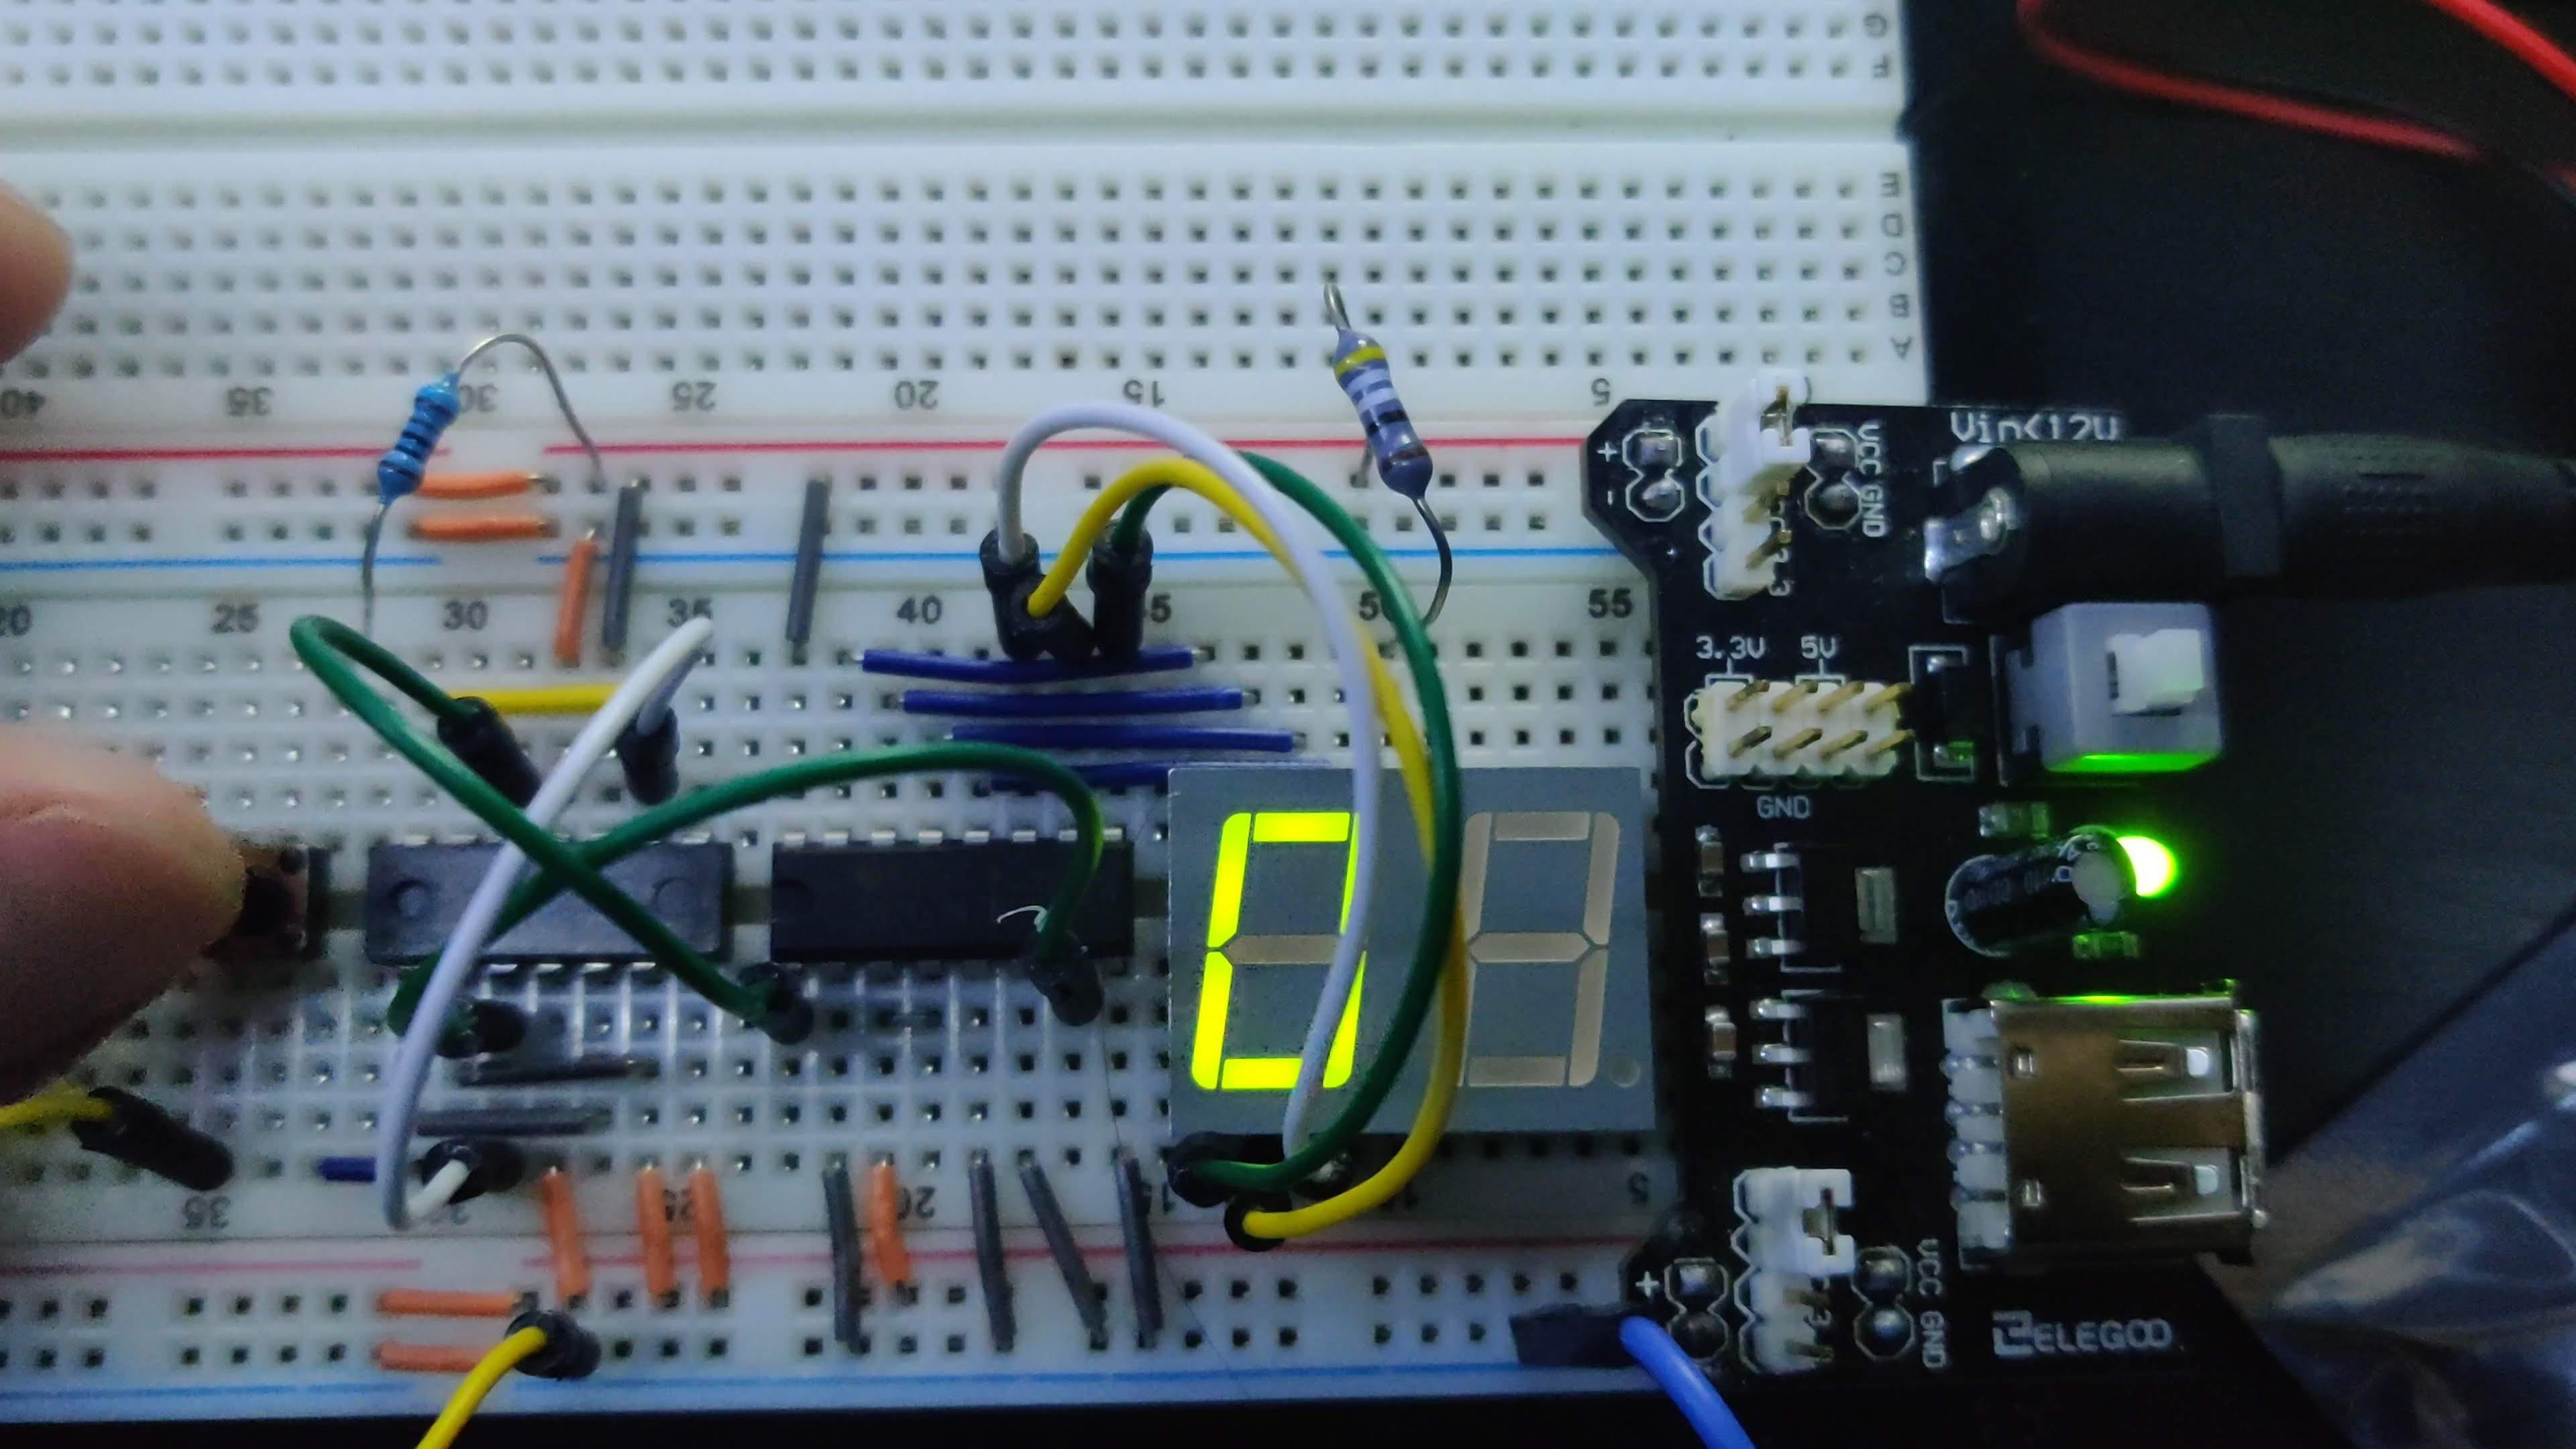
\includegraphics[width=\textwidth]{ECE2300L_Lab11_0.jpg}
\end{figure}
\begin{figure}[ht!]
  \centering
  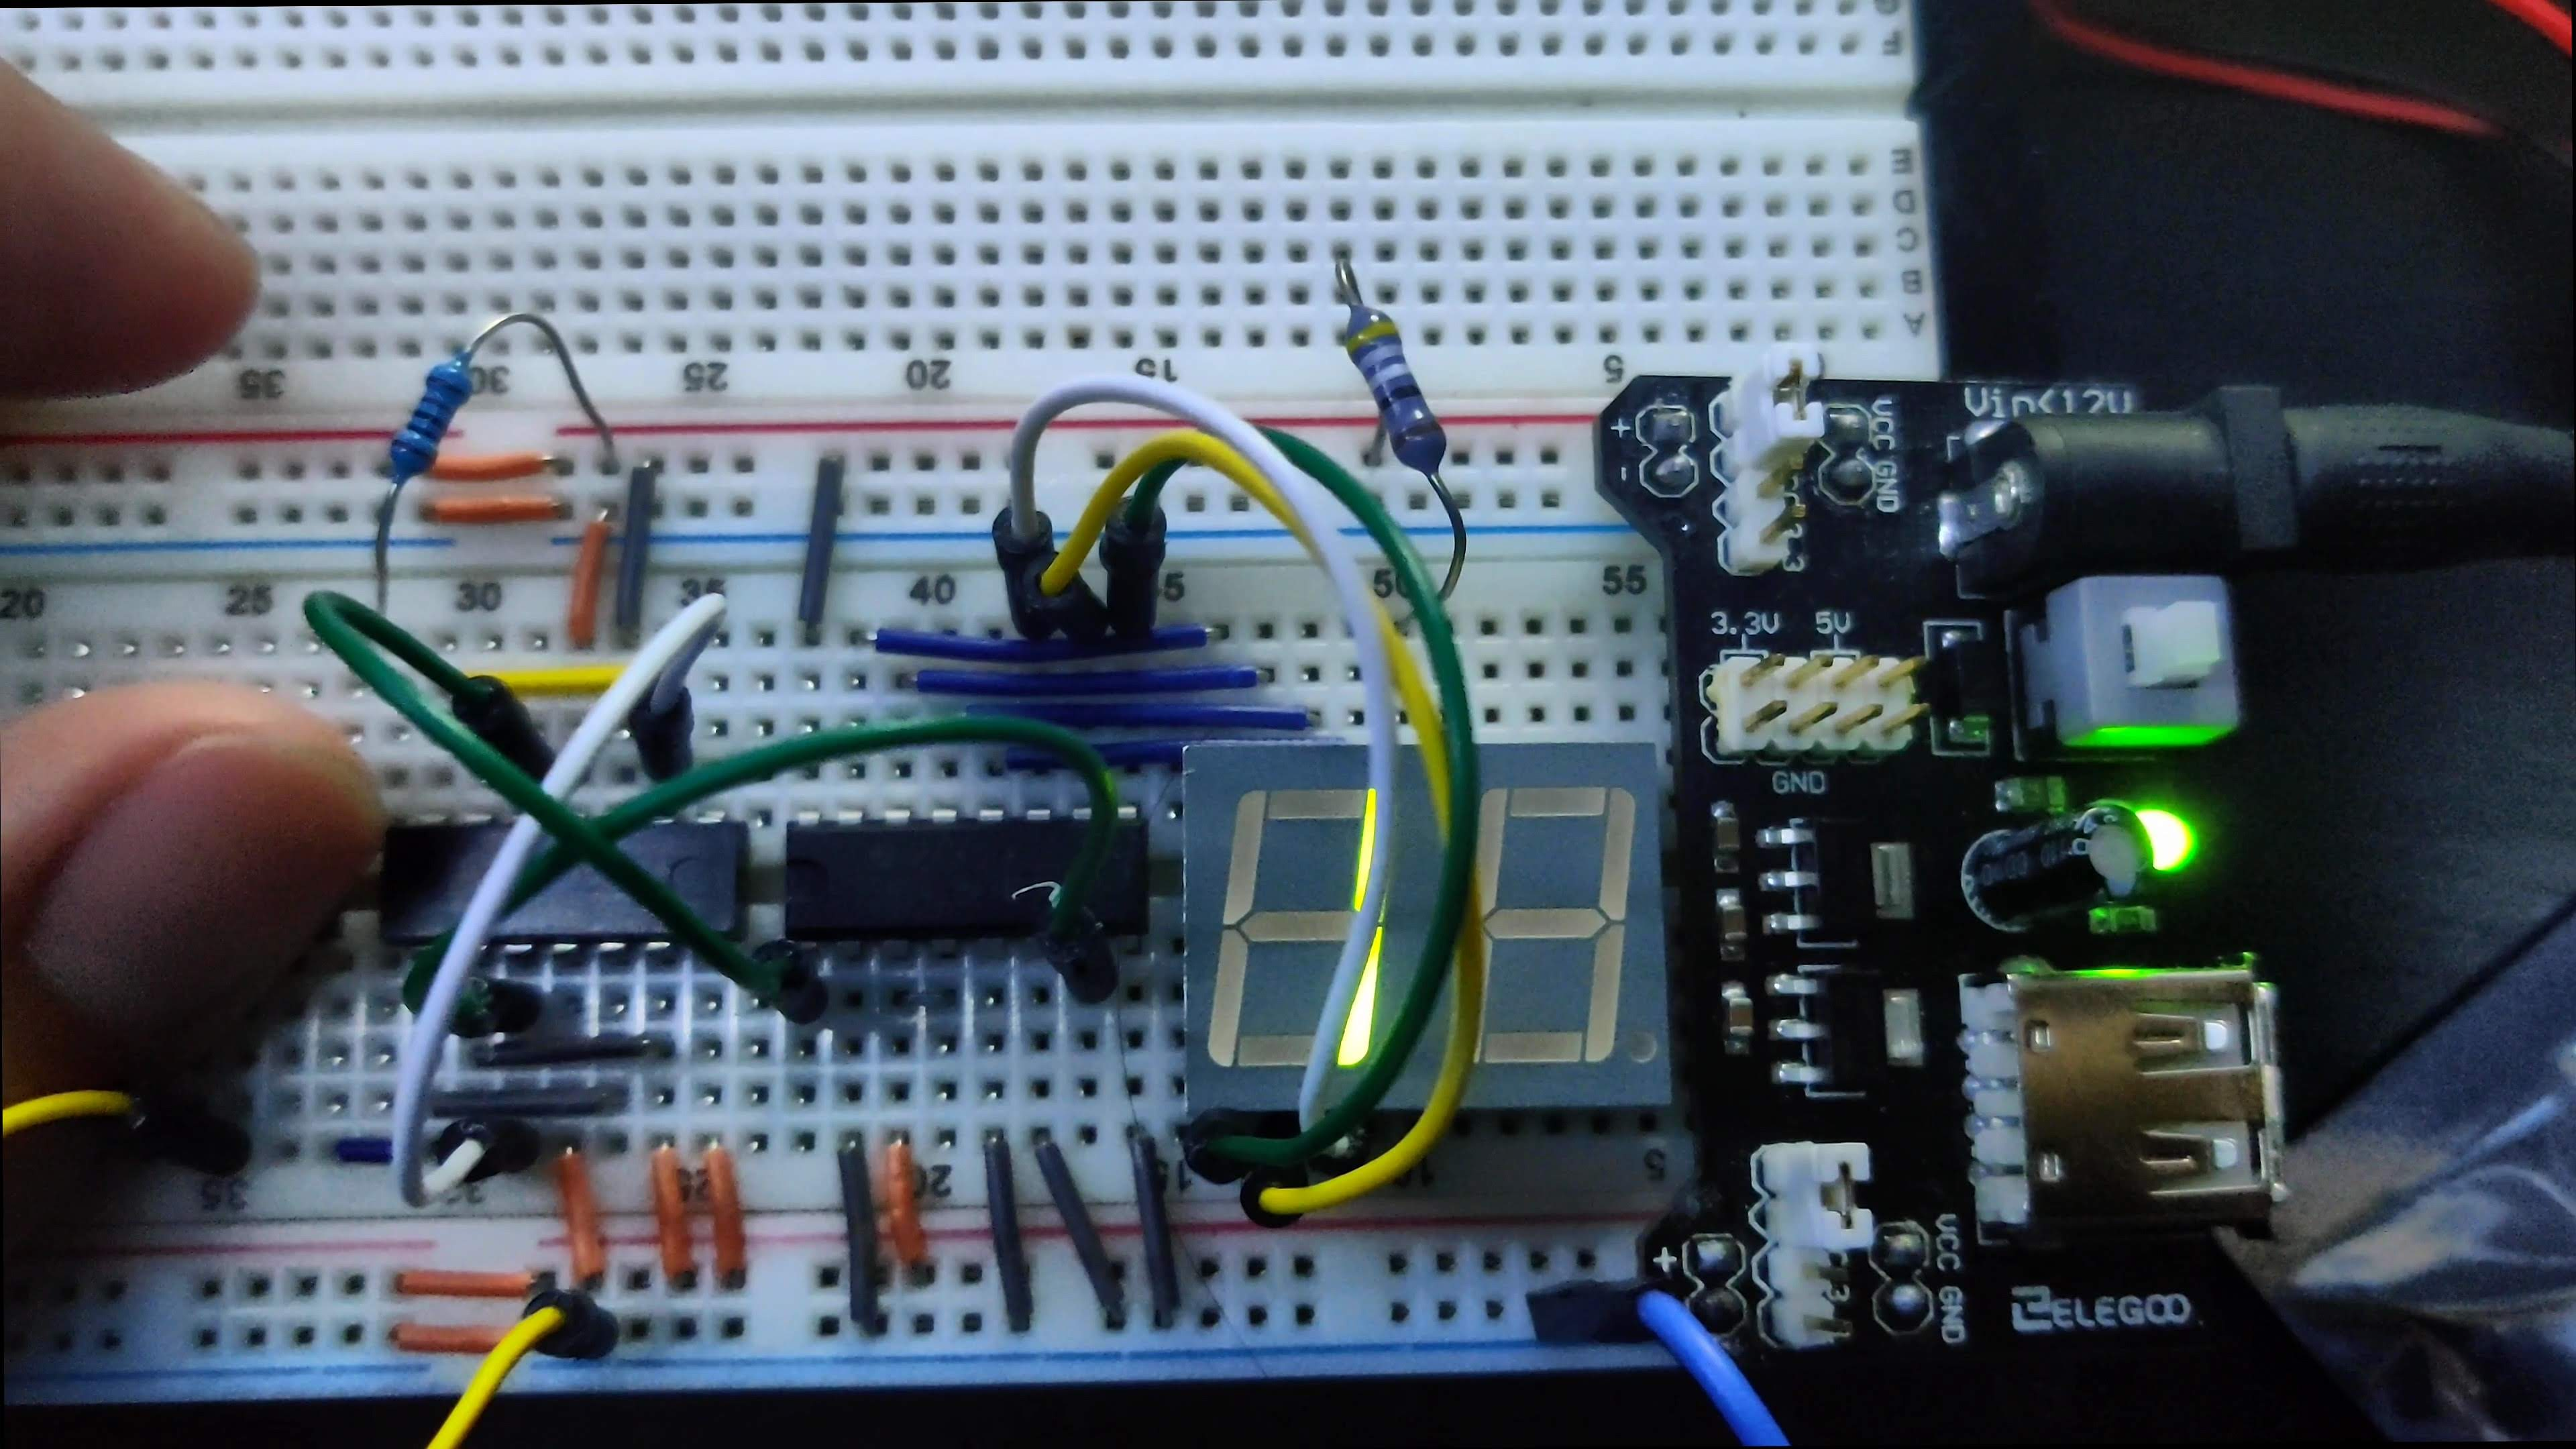
\includegraphics[width=\textwidth]{ECE2300L_Lab11_1.jpg}
\end{figure}
\begin{figure}[ht!]
  \centering
  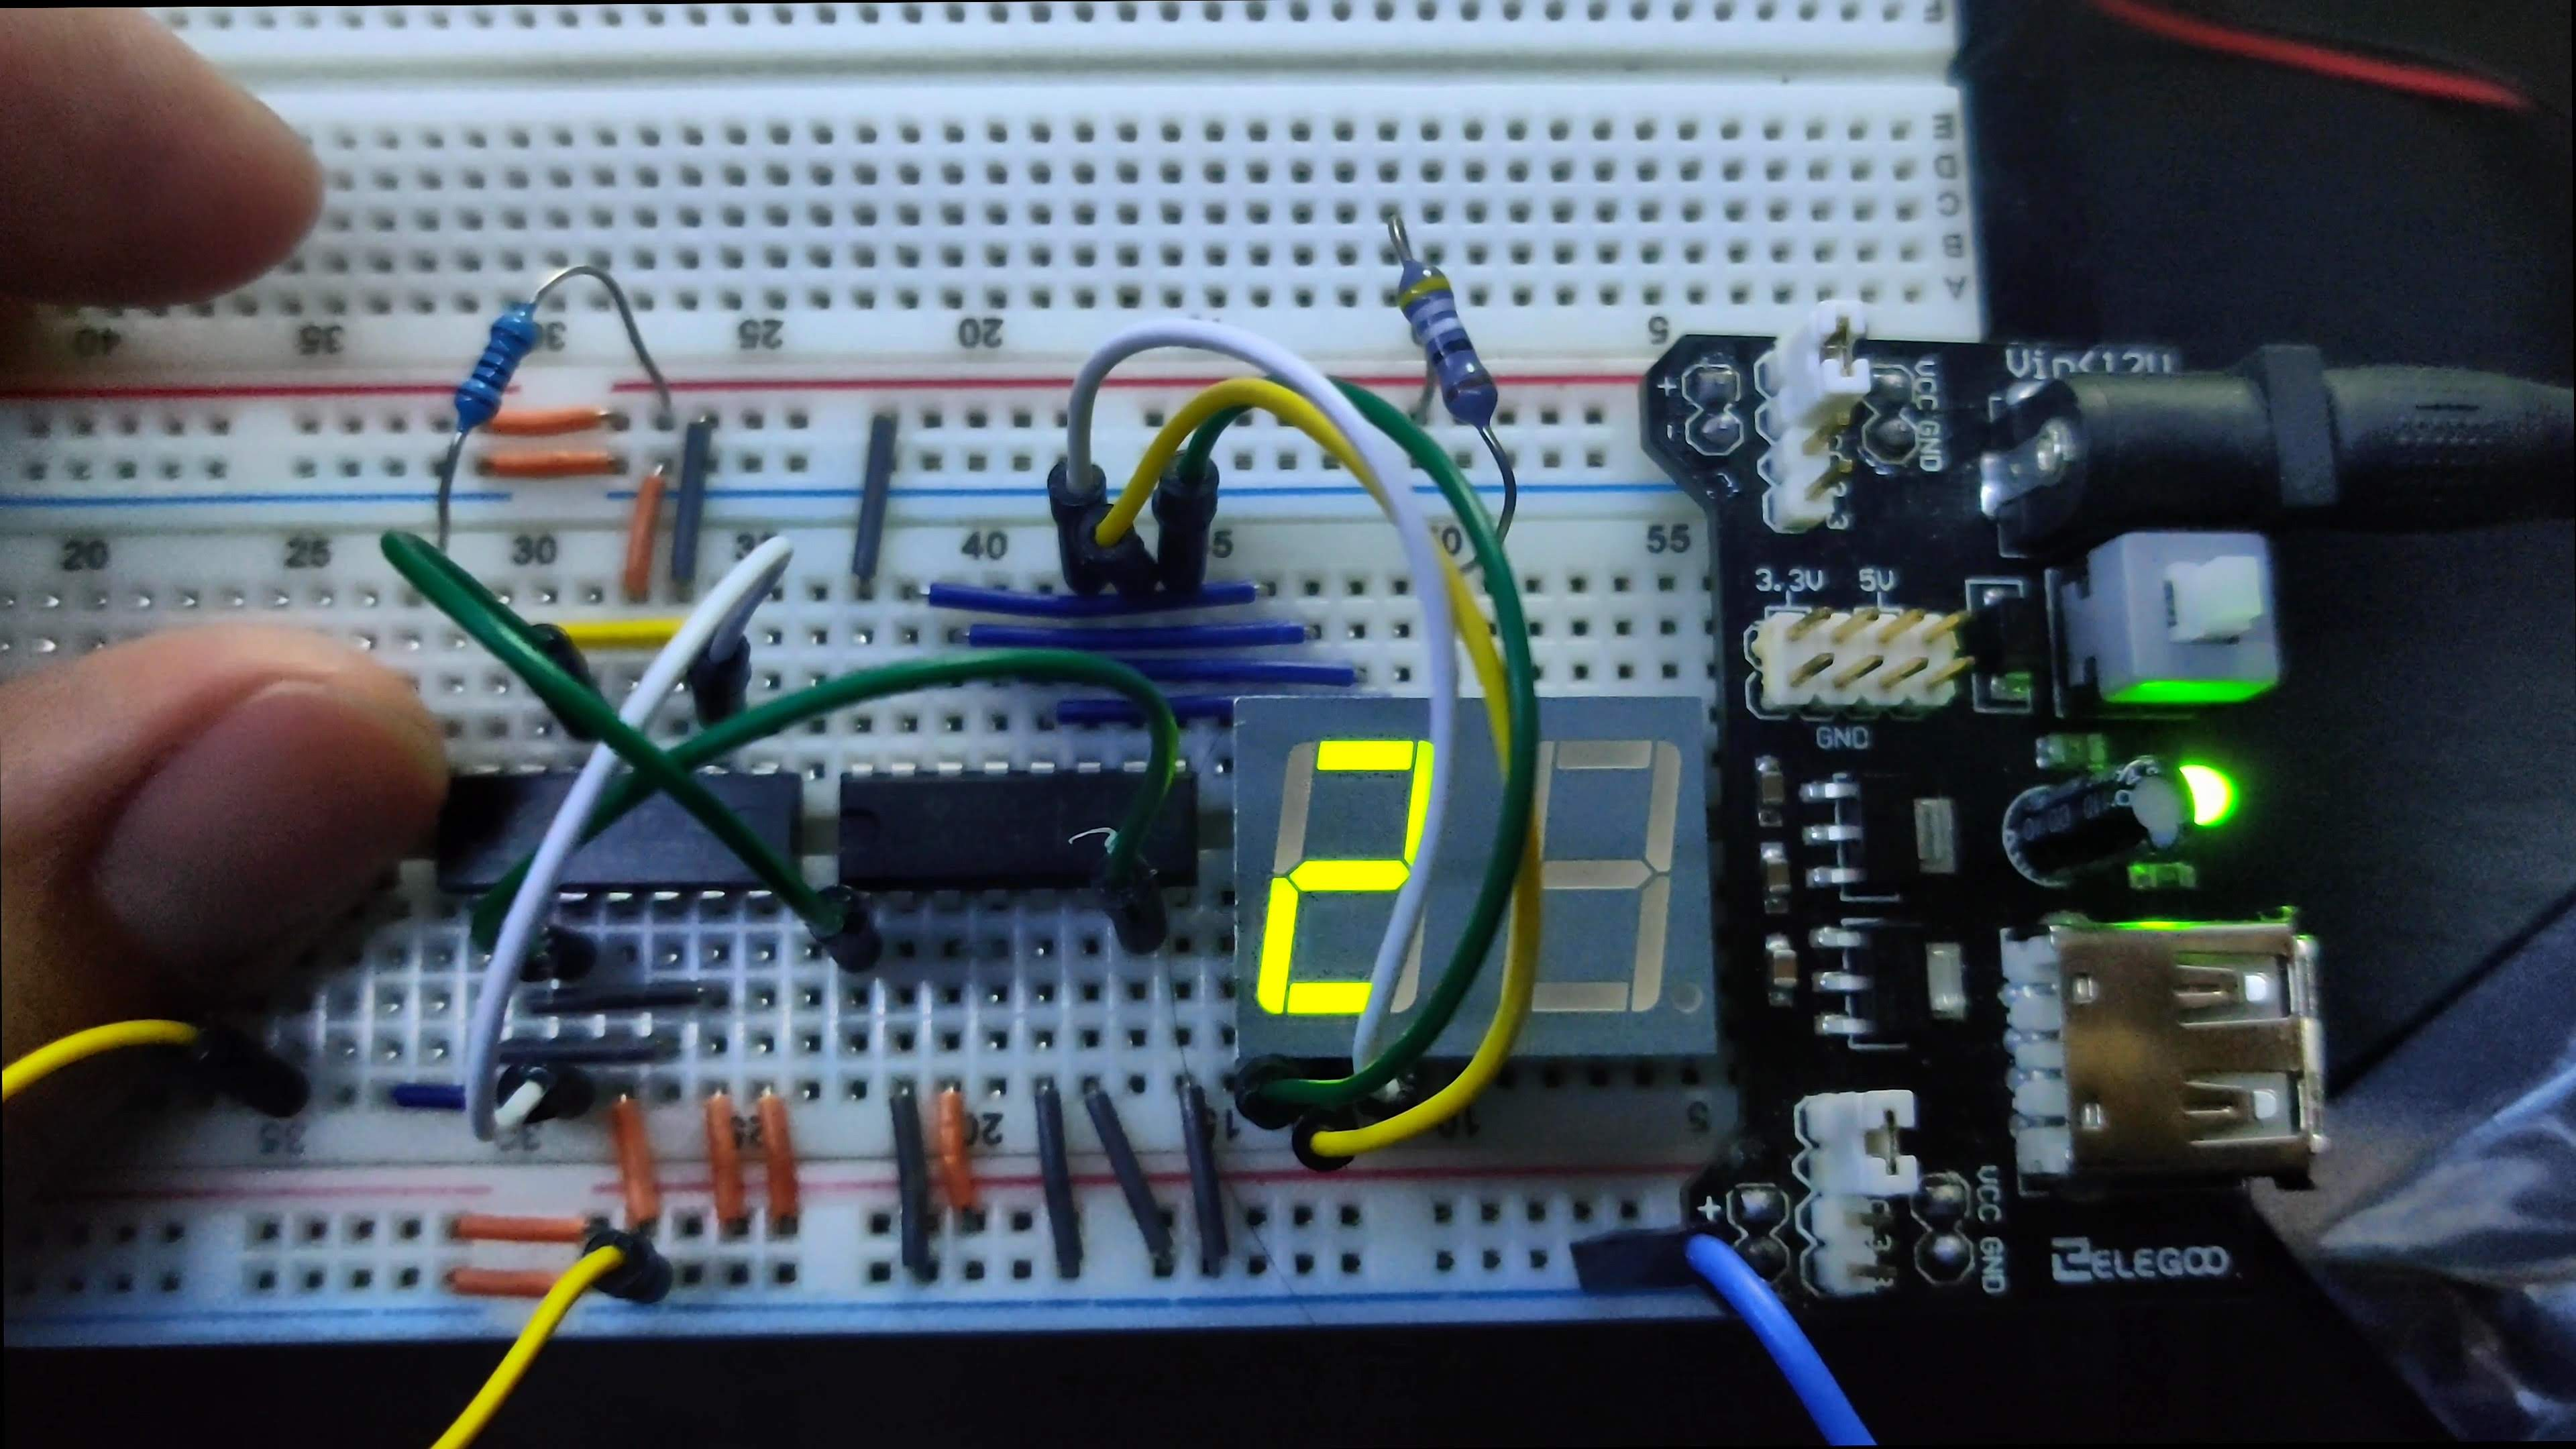
\includegraphics[width=\textwidth]{ECE2300L_Lab11_2.jpg}
\end{figure}
\begin{figure}[ht!]
  \centering
  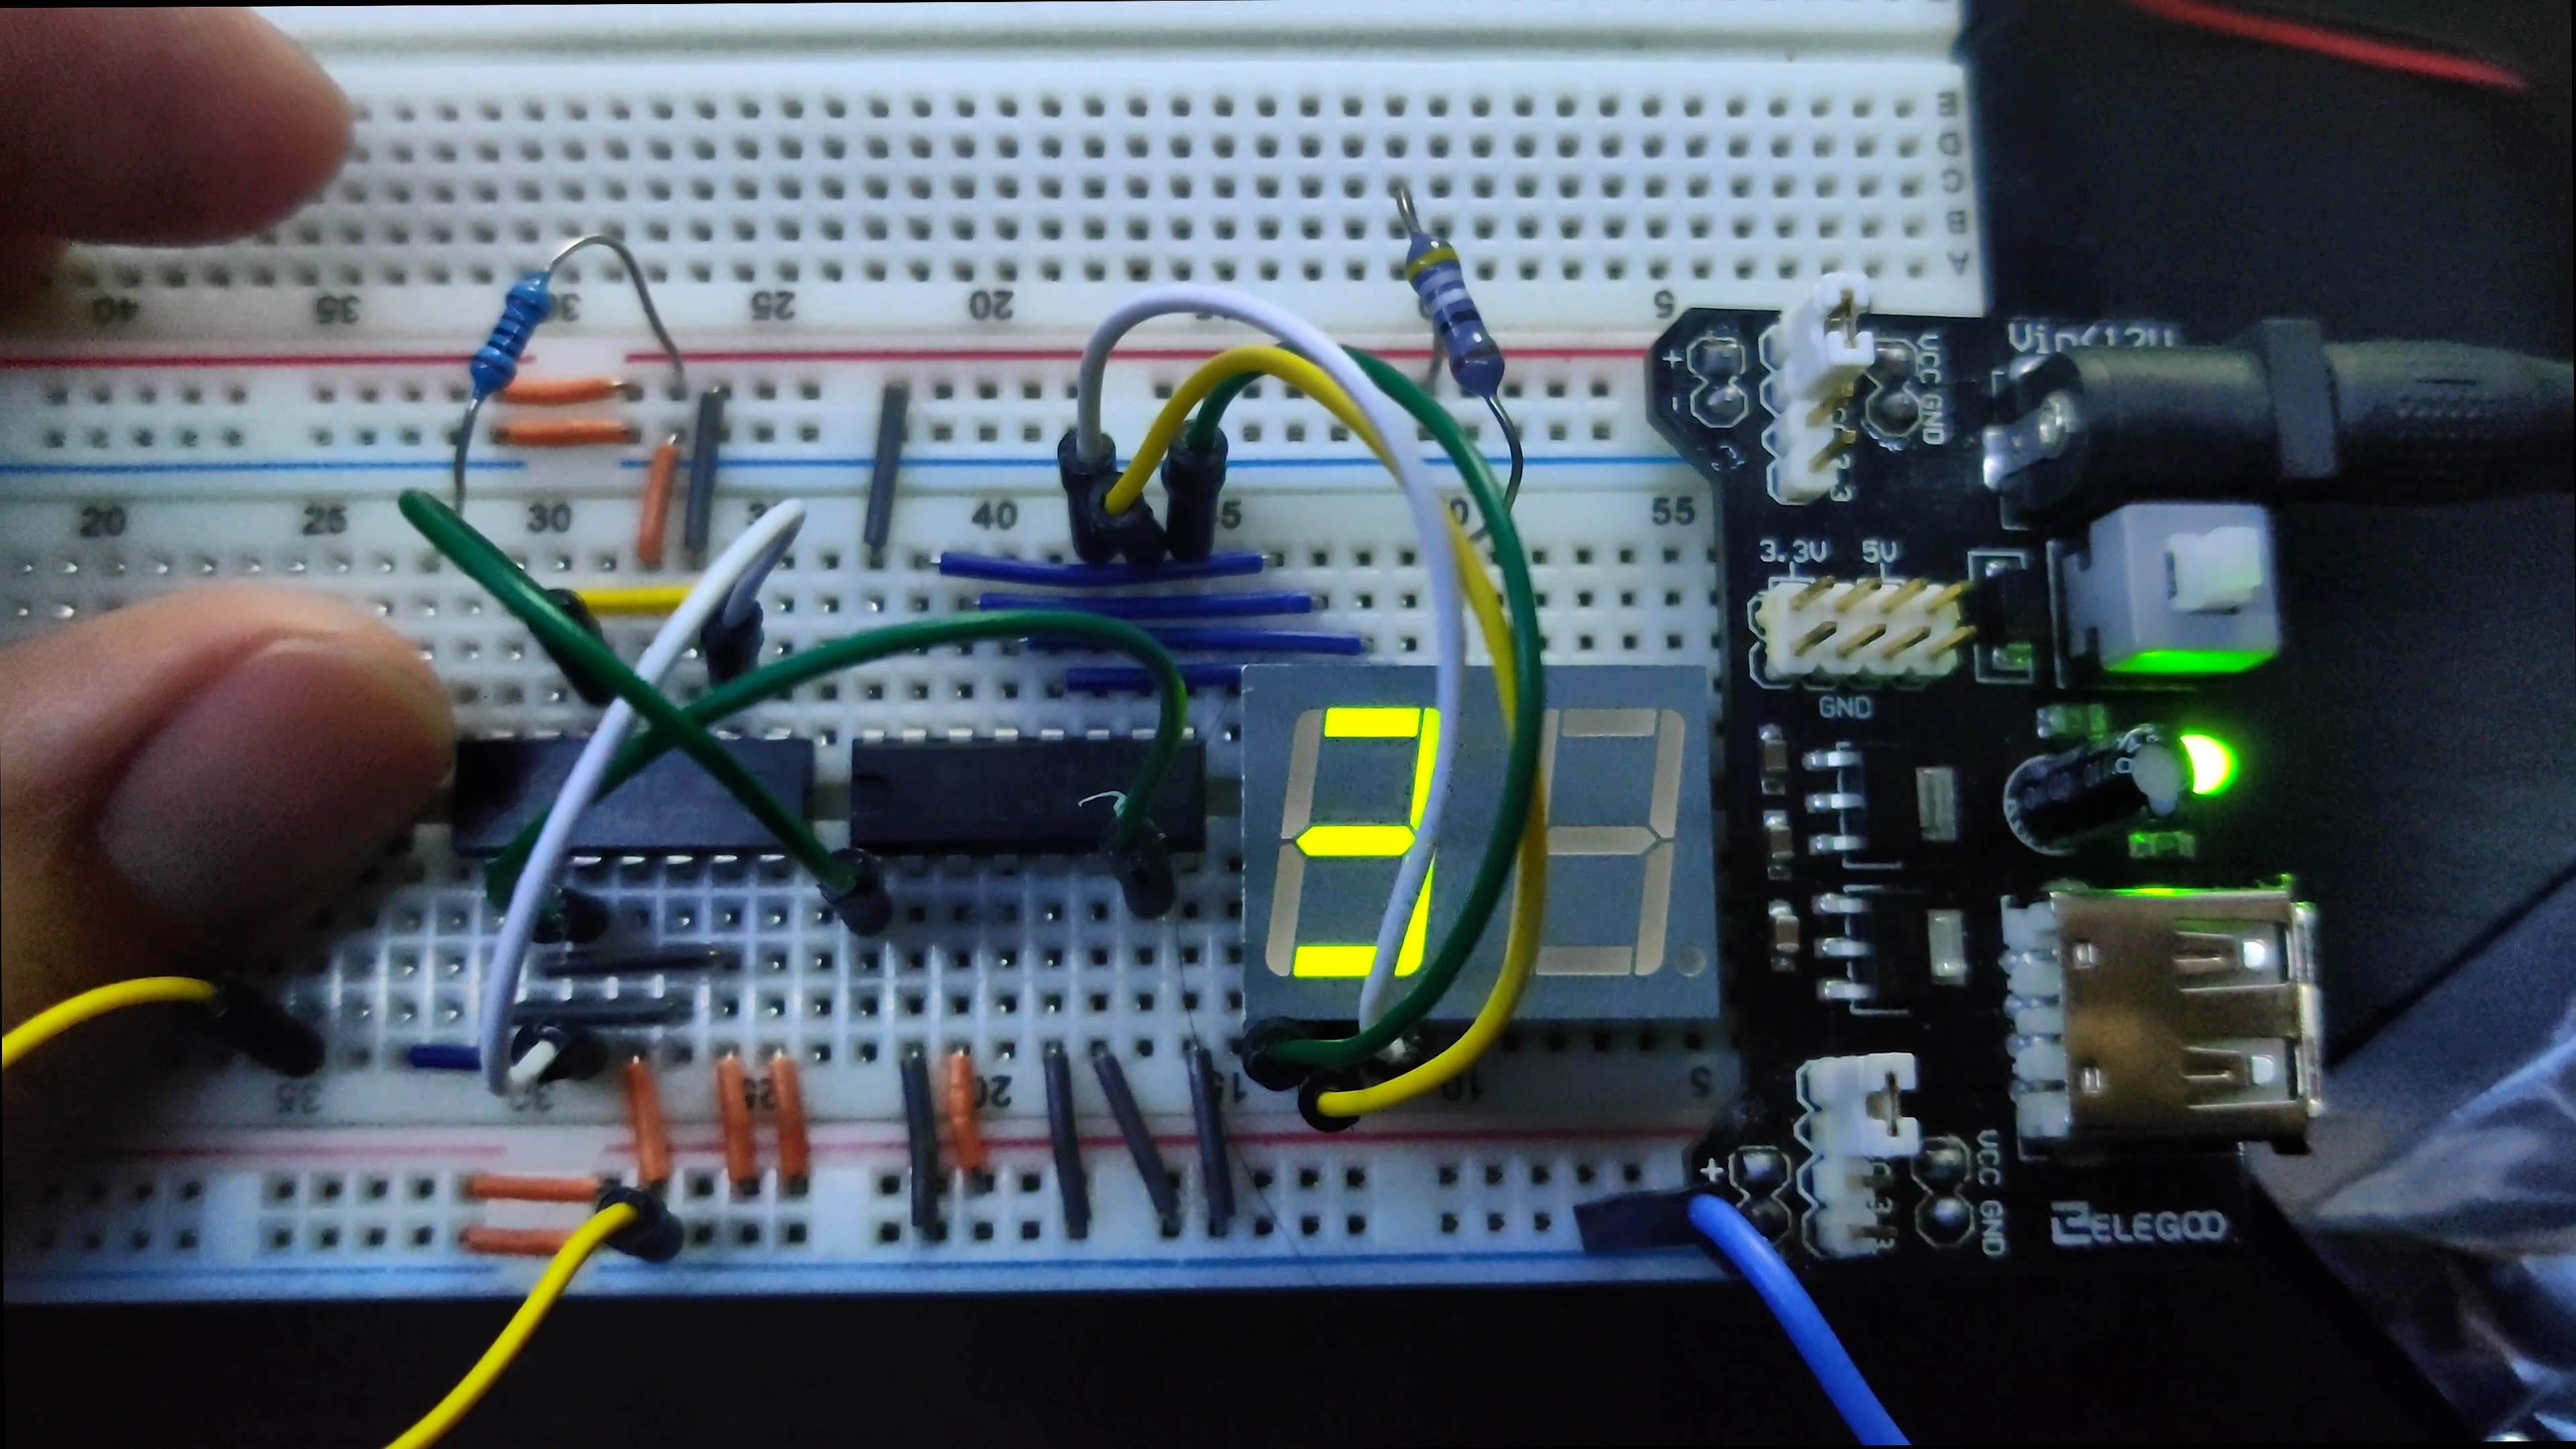
\includegraphics[width=\textwidth]{ECE2300L_Lab11_3.jpg}
\end{figure}
\end{document}
